\documentclass[11pt, oneside]{article}
\usepackage[letterpaper, margin=2cm]{geometry}
\usepackage{MATH520}

\begin{document}
\noindent \textbf{\Large{Caleb Logemann \\
MATH 520 Methods of Applied Math II \\
Homework 9
}}

\subsection*{Section 14.5}
\begin{enumerate}
  \item[\#5] % Done
    Let $Lu = a_2(x) u'' + a_1(x)u' + a_0(x) u$ with $a_2' = a$, so that $L$ is
    formally self adjoint.
    If $B_1 u = C_1 u(a) + C_2u'(a)$, $B_2 u = C_3u(b) + C_4u'(b)$, show that
    $\set{B_1^*, B_2^*} = \set{B_1, B_2}$.

    \begin{proof}
      Consider the operators $B_1^* \psi = C_1 \psi(a) + C_2 \psi'(a) = B_1 \psi$
      and $B_2^* \psi = C_3 \psi(b) + C_4 \psi'(b) = B_2 \psi$.
      In order to show that $\set{B_1^*, B_2^*}$ is adjoint to $\set{B_1, B_2}$
      it must be shown that
      \[
        \eval{J(\phi, \psi)}{a}{b} = 0
      \]
      whenever $B_1 \phi = B_2 \phi = B_1^* \psi = B_2^* \psi = 0$.

      Therefore let $\phi$ and $\psi$ be chosen such that
      \[
        B_1 \phi = B_2 \phi = B_1^* \psi = B_2^* \psi = 0.
      \]

      First consider $B_1 \phi = B_1^* \psi = 0$.
      These equations can be rewritten as
      \begin{align*}
        C_1 \phi(a) &= - C_2 \phi'(a) \\
        C_1 \psi(a) &= - C_2 \psi'(a).
      \end{align*}
      Multiplying these equations gives
      \begin{align*}
        -C_1 C_2 \phi(a) \psi'(a) &= -C_1 C_2 \psi(a) \phi'(a)
        \intertext{or}
        \phi(a) \psi'(a) - \phi'(a) \psi(a) &= 0
      \end{align*}
      Note that this statement is still true if one of $C_1$ or $C_2$ is
      zero.
      If one of them is zero, then either $\phi(a) = \psi(a) = 0$ or
      $\phi'(a) = \psi'(a) = 0$, which still gives
      \[
        \phi(a) \psi'(a) - \phi'(a) \psi(a) = 0 - 0 = 0
      \]

      Similary with $B_2 \phi = B_2^* \psi = 0$, it is possible to rewrite
      these equations as
      \begin{align*}
        C_3 \phi(b) &= - C_4 \phi'(b) \\
        C_3 \psi(b) &= - C_4 \psi'(b).
      \end{align*}
      Multiplying these equations gives
      \begin{align*}
        -C_3 C_4 \phi(b) \psi'(b) &= -C_3 C_4 \psi(b) \phi'(b)
        \intertext{or}
        \phi(b) \psi'(b) - \phi'(b) \psi(b) &= 0
      \end{align*}
      Again if $C_3$ or $C_4$ is zero, then $\phi(b) = \psi(b) = 0$ or
      $\phi'(b) = \psi'(a) = 0$ which implies
      \[
        \phi(b) \psi'(b) - \phi'(b) \psi(b) = 0
      \]

      Now consider the boundary functional $J(\phi, \psi)$.
      The boundary function $J(\phi, \psi)$ can be fully expressed as
      \[
        J(\phi, \psi) = a_2\p{\phi' \psi - \phi \psi'} + (a_1 - a_2') \phi \psi.
      \]
      Since the differential operator is formally self-adjoint, $a_1 = a_2'$, so
      this is equivalent to
      \[
        J(\phi, \psi) = a_2\p{\phi' \psi - \phi \psi'}
      \]

      Now the condition $\eval{J(\phi, \psi)}{a}{b} = 0$ is equivalent to
      \[
        a_2\p{\phi'(b) \psi(b) - \phi(b) \psi'(b)} - a_2\p{\phi'(a) \psi(a) - \phi(a) \psi'(a)} = 0.
      \]
      Since we have already shown that $\phi'(b) \psi(b) - \phi(b) \psi'(b) = 0$
      and $\phi'(a) \psi(a) - \phi(a) \psi'(a) = 0$ when the boundary operators
      are met.
      This condition is cleary met, when $B_1 \phi = B_2 \phi = B_1^* \psi = B_2^* \psi = 0$.

      Therefore $\set{B_1^*, B_2^*}$ is adjoint to $\set{B_1, B_2}$ and since
      $B_1 = B_1^*$ and $B_2 = B_2^*$ this implies that
      $\set{B_1^*, B_2^*} = \set{B_1, B_2}$.
      In other words $\set{B_1, B_2}$ is adjoint to itself.
      The purpose of this exercise is to show that a formally self-adjoint
      differential operator with boundary conditions of the form found in $B_1$
      and $B_2$ forms a self-adjoint linear operator.
    \end{proof}

  \pagebreak
  \item[\#8]
    When we rewrite $a_2(x) u'' + a_1(x) u' + a_0(x) u = \lambda u$ as
    \[
      -(p(x)u')' + q(x)u = \lambda \rho(x) u
    \]
    the latter is often referred to as the \textit{Liouville normal form}.
    Consider the eigenvalue problem
    \[
      x^2 u'' + xu' + u = \lambda u \qquad 1 < x < 2
    \]
    \[
      u(1) = u(2) = 0
    \]
    \begin{enumerate}
      \item[(a)] % Done
        Find the Liouville normal form.

        In order to find the Liouville normal form, the function $a_2(x)$ must
        be strictly less than zero, so I will first rewrite this eigenvalue
        problem as
        \[
          -x^2 u'' - xu' - u = -\lambda u \qquad 1 < x < 2
        \]
        \[
          u(1) = u(2) = 0
        \]
        The functions $p(x)$, $\rho(x)$, and $q(x)$ can be found as follows.
        \begin{align*}
          p(x) &= \exp\p{\dintt{a}{x}{\frac{a_1(s)}{a_2(s)}}{s}} \\
          &= \exp\p{\dintt{a}{x}{\frac{-s}{-s^2}}{s}} \\
          &= \exp\p{\dintt{a}{x}{\frac{1}{s}}{s}} \\
          &= \exp\p{\eval{\ln{s}}{s = a}{x}} \\
          &= e^{\ln{x} - \ln{a}} \\
          &= e^{\ln{\frac{x}{a}}} \\
          &= \frac{x}{a} \\
          \rho(x) &= - \frac{p(x)}{a_2(x)} \\
          &= - \frac{x/a}{-x^2} \\
          &= \frac{1}{ax} \\
          q(x) &= a_0(x) \rho(x) \\
          &= (-1)\frac{1}{ax}\\
          &= -\frac{1}{ax}\\
        \end{align*}
        Therefore the Liouville normal form of this eigenvalue problem is
        \[
          -\p{\frac{x}{a} \phi'}' - \frac{1}{ax} \phi = -\lambda \frac{1}{ax} \phi
        \]
        or
        \[
          \p{\frac{x}{a} \phi'}' + \frac{1}{ax} \phi = \lambda \frac{1}{ax} \phi
        \]

      \item[(b)] % Done
        What is the orthogonality relationship satisfied by the eigenfunctions?

        The eigenfunctions of this linear operator satisfy an orthogonality
        relationship with respect to the weight $\rho$.
        In mathematical terms,
        \[
          \dintt{a}{b}{\phi_n(x) \phi_m(x) \rho(x)}{x} =
          \begin{cases}
            0 & n \neq m \\
            1 & n = m
          \end{cases}
        \]
        or
        \[
          \dintt{a}{b}{\frac{\phi_n(x) \phi_m(x)}{ax}}{x} =
          \begin{cases}
            0 & n \neq m \\
            1 & n = m
          \end{cases}
        \]

      \item[(c)]
        Find the eigenvalues and eigenfunctions.
        (You may find the original form of the equation easier to work with than
        the Liouville normal form when computing the eigenvalues and
        eigenfunctions.)

        The original differential equation is a Cauchy-Euler differential
        equation.
        As such I will guess solutions in the form $u(x) = x^m$.
        \begin{align*}
          x^2 m(m - 1) x^{m - 2} + x m x^{m - 1} + (1 - \lambda) x^m &= 0 \\ 
          m(m - 1) x^m + m x^m + (1 - \lambda) x^m &= 0 \\ 
          \p{m(m - 1) + m + (1 - \lambda)} x^m &= 0 \\ 
          m(m - 1) + m + (1 - \lambda) &= 0 \\ 
          m^2 - m + m + 1 - \lambda &= 0 \\ 
          m^2 + 1 - \lambda &= 0 \\ 
          m^2 + 1 - \lambda &= 0 \\ 
          m^2 &= \lambda - 1
        \end{align*}
        If $\lambda \in \RR$ and $\lambda > 1$, then the general solution is
        \[
          u(x) = c_1 x^{\sqrt{\lambda - 1}} + c_2 x^{-\sqrt{\lambda - 1}}
        \]
        Using the boundary conditions implies that
        \begin{align*}
          u(1) = c_1 + c_2 = 0 \\
          u(2) = c_1 2^{\sqrt{\lambda - 1}} + c_2 2^{-\sqrt{\lambda - 1}} = 0\\
          c_1 = -c_2 \\
          -c_2 2^{\sqrt{\lambda - 1}} + c_2 2^{-\sqrt{\lambda - 1}} = 0
          c_2 = 0 \\
          c_1 = 0
        \end{align*}
        This results in the trivial solution, so $\lambda > 1$ is not an
        eigenvalue.

        If $\lambda = 1$, then the general solution is
        \[
          u(x) = c_1 \ln{x} + c_2
        \]
        Applying the boundary conditions gives
        \begin{align*}
          u(1) = c_2 = 0 \\
          u(2) = c_1 \ln{2} = 0 \\
          c_1 = 0
        \end{align*}
        This is also the trivial solution so $\lambda = 1$ is not an eigenvalue.

        If $\lambda < 1$ or $\lambda \in \CC$ with nonzero imaginary component,
        then $m = \sqrt{\lambda - 1}$ is complex.
        In this case let $\alpha = Re(\sqrt{\lambda - 1})$ and
        $\beta = Im(\sqrt{\lambda - 1}$.
        Then the general solution is
        \[
          u(x) = c_1 x^{\alpha} \cos{\beta \ln{x}} + c_2 x^{\alpha} \sin{\beta \ln{x}}
        \]
        Applying the boundary conditions gives.
        \begin{align*}
          u(1) &= c_1 \cos{0} + c_2 \sin{0} \\
          &= c_1 = 0 \\
          u(2) &= c_2 2^{\alpha} \sin{\beta \ln{2}} = 0 \\
          c_2 &= 0
        \end{align*}
        Again this is the trivial solution.
        Therefore there are no eigenvalues and eigenfunctions for this
        differential equation.
    \end{enumerate}

  \pagebreak
  \item[\#10]
    Consider the Sturm-Liouville problem
    \begin{align*}
      u'' + \lambda u = 0 \qquad 0 < x < 1 \\
      u(0) - u'(0) = u(1) = 0
    \end{align*}
    \begin{enumerate}
      \item[(a)] % Done
        Multiply the equation by $u$ and integrate by parts to show that any
        eigenvalue is positive.

        First I will note a few useful facts, first since $u(0) - u'(0) = 0$,
        this implies that $u(0) = u'(0)$.
        Also if $u$ is nontrivial this guarantees that
        $\dintt{0}{1}{u^2(x)}{x} > 0$.
        Finally if $u$ is a nontrivial solution then $u'(x) \neq 0$ as
        $u(1) = 0$ makes any constant function is zero.
        This shows that $\dintt{0}{1}{\p{u'(x)}^2}{x} > 0$ as well.

        Multiplying by $u$ gives the following equation
        \[
          uu'' + \lambda u^2 = 0.
        \]
        Integrating both sides over $\br{0, 1}$ gives
        \[
          \dintt{0}{1}{u(x)u''(x)}{x} + \lambda \dintt{0}{1}{u^2(x)}{x} = \dintt{0}{1}{0}{x}
        \]
        This can be simplified using integration by parts
        \begin{align*}
          \dintt{0}{1}{u(x)u''(x)}{x} + \lambda \dintt{0}{1}{u^2(x)}{x} &= 0 \\
          \eval{u(x)u'(x)}{x = 0}{1} - \dintt{0}{1}{\p{u'(x)}^2}{x} + \lambda \dintt{0}{1}{u^2(x)}{x} &= 0 \\
          u(1)u'(1) - u(0)u'(0) - \dintt{0}{1}{\p{u'(x)}^2}{x} + \lambda \dintt{0}{1}{u^2(x)}{x} &= 0
          \intertext{Since $u(1) = 0$ and $u(0) = u'(0)$}
           -u^2(0) - \dintt{0}{1}{\p{u'(x)}^2}{x} + \lambda \dintt{0}{1}{u^2(x)}{x} &= 0.
        \end{align*}
        Since $\dintt{0}{1}{u^2(x)}{x} > 0$
        \[
          \lambda = \frac{u^2(0) + \dintt{0}{1}{\p{u'(x)}^2}{x}}{\dintt{0}{1}{u^2(x)}{x}} > 0.
        \]

      \item[(b)]
        Show that the eigenvalues are the positive solutions of
        $\tan{\sqrt{\lambda}} = - \sqrt{\lambda}$.

        Didn't have time to finish.

      \item[(c)] % Done
        Show graphically that such roots exist, and form an infinite sequence
        $\lambda_k$ such that $(k - 1/2)\pi < \sqrt{\lambda_k} < k \pi$ and
        \[
          \lim[k \to \infty]{\sqrt{\lambda_k} - (k - 1/2)\pi} = 0
        \]

        First this graph shows that solutions to the equation
        $\tan{\sqrt{\lambda}} = -\sqrt{\lambda}$ exist.
        \begin{center}
          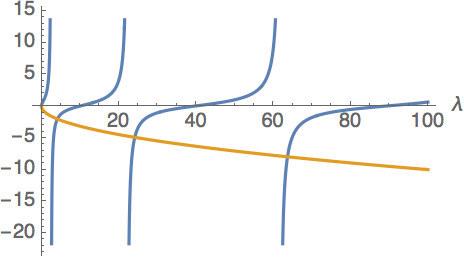
\includegraphics[scale=.5]{Figures/09_1}
        \end{center}

        Next consider the sequence $\lambda_k = \p{(k - 1/2)\pi + \frac{1}{k}}^2$
        meets these criterion.
        Note that $\sqrt{\lambda_k} = (k - 1/2)\pi + \frac{1}{k}$.
        Clearly $\sqrt{\lambda_k} > (k - 1/2)\pi$ and $\sqrt{\lambda_k} < k\pi$
        as $\frac{1}{k} < \frac{\pi}{2}$.

        Also
        \begin{align*}
          \lim[k \to \infty]{\sqrt{\lambda_k} - (k - 1/2)\pi} &= \lim[k \to \infty]{(k - 1/2)\pi + \frac{1}{k} - (k - 1/2)\pi} \\
          &= \lim[k \to \infty]{\frac{1}{k}} = 0
        \end{align*}
    \end{enumerate}

  \pagebreak
  \item[\#14] % Done
    If $\set{\psi_n}_{n = 1}^{\infty}$ are Dirichlet eigenfunctions of the
    Laplacian making up an orthonormal basis of $L^2(\Omega)$, let
    $\zeta_n = \psi_n/\sqrt{\lambda_n}$
    ($\lambda_n$ the corresponding eigenvalue).
    \begin{enumerate}
      \item[(a)] % Done
        Show that $\set{\zeta_n}_{n = 1}^{\infty}$ is an orthonormal basis of
        $H^1_0(\Omega)$.

        \begin{proof}
          First I will show that $\zeta_n$ is an orthonormal set.
          In order to do this I will use that fact that
          \[
            \dintt{\Omega}{}{\nabla u \nabla v}{x} = \lambda \dintt{\Omega}{}{u v}{x}
          \]
          for any $v \in H_0^1(\Omega)$ where $\lambda$ and $u$ are a Dirichlet
          eigenvalue and eigenvector pair for the Laplacian on $\Omega$.

          Consider $\abr[H_0^1(\Omega)]{\zeta_n, \zeta_m}$
          \begin{align*}
            \abr[H_0^1(\Omega)]{\zeta_n, \zeta_m} &= \dintt{\Omega}{}{\nabla \zeta_n \cdot \nabla \zeta_m}{x} \\
            &= \frac{1}{\sqrt{\lambda_n \lambda_m}}\dintt{\Omega}{}{\nabla \psi_n \cdot \nabla \psi_m}{x}
            \intertext{Since $\psi_m \in H^1_0(\Omega)$ and $\psi_n$ an
              eigenfunction}
            &= \frac{\lambda_n}{\sqrt{\lambda_n \lambda_m}}\dintt{\Omega}{}{\psi_n \psi_m}{x} \\
            &= \frac{\lambda_n}{\sqrt{\lambda_n \lambda_m}} \abr[L^2(\Omega)]{\psi_n, \psi_m}.
            \intertext{Since $\set{\psi}$ already forms an orthonormal basis of
              $L^2$, so}
            &= \frac{\lambda_n}{\sqrt{\lambda_n \lambda_m}} \delta_{nm}
          \end{align*}
          where $\delta_{nm}$ is the Kronecker delta.
          This shows that if $n = m$, then
          $\abr[H_0^1(\Omega)]{\zeta_n, \zeta_m} = 1$ and if $n \neq m$, then
          $\abr[H_0^1(\Omega)]{\zeta_n, \zeta_m} = 0$.
          This shows that $\set{\zeta_n}$ is an orthonormal set in
          $H^1_0(\Omega)$.

          Now I will show that $\set{\zeta_n}$ is a basis of $H^1_0(\Omega)$.
          In order to show that this is a basis, I will show that this set is
          complete in $H^1_0(\Omega)$ or equivalently that the zero function is
          the only function orthogonal to the entire set.
          Therefore let $u \in H^1_0(\Omega)$, such that
          \[
            \abr[H^1_0(\Omega)]{\zeta_n, u} = 0
          \]
          for all $n \in \NN$.
          \begin{align*}
            0 &= \abr[H^1_0(\Omega)]{\zeta_n, u} \\
            &= \dintt{\Omega}{}{\nabla \zeta_n \cdot \nabla u}{x} \\
            &= \frac{1}{\sqrt{\lambda_n}}\dintt{\Omega}{}{\nabla \psi_n \cdot \nabla u}{x}
            \intertext{Since $u \in H^1_0(\Omega)$ and $\psi_n$ is a Dirichlet
              eigenfunction.}
            &= \frac{\lambda_n}{\sqrt{\lambda_n}}\dintt{\Omega}{}{\psi_n u}{x} \\
            &= \frac{\lambda_n}{\sqrt{\lambda_n}} \abr[L^2(\Omega)]{\psi_n, u}
          \end{align*}
          This shows that $\abr[L^2(\Omega)]{\psi_n, u} = 0$ for all $n$.
          Since $\set{\psi_n}$ is already a basis of $L^2$ this means that
          $u = 0$.
          Therefore $\set{\zeta_n}$ is complete in $H^1_0(\Omega)$ and thus
          is a basis of $H^1_0(\Omega)$.
        \end{proof}

      \item[(b)] % Done
        Show that $f \in H_0^1(\Omega)$ if and only if
        $\sum{n = 1}{\infty}{\lambda_n \abs{\abr{f, \psi_n}}^2} < \infty$

        \begin{proof}
          First I will do some manipulation on the given sum.
          \begin{align*}
            \sum{n = 1}{\infty}{\lambda_n \abs{\abr{f, \psi_n}}^2} &= \sum{n = 1}{\infty}{\lambda_n \abs{\dintt{\Omega}{}{f \psi_n}{x}}^2} \\
            &= \sum{n = 1}{\infty}{\frac{1}{\lambda_n} \abs{\dintt{\Omega}{}{f \lambda_n \psi_n}{x}}^2}
            \intertext{Since $\psi_n$ and $\lambda_n$ are an eigenfunction and
              eigenvalue pair for the Laplacian}
            &= \sum{n = 1}{\infty}{\frac{1}{\lambda_n} \abs{\dintt{\Omega}{}{f \Delta \psi_n}{x}}^2} \\
            &= \sum{n = 1}{\infty}{\frac{1}{\lambda_n} \abs{\dintt{\Omega}{}{\nabla f \nabla \psi_n}{x}}^2} \\
            &= \sum{n = 1}{\infty}{\frac{1}{\lambda_n} \abs{\abr[H^1_0(\Omega)]{f, \psi_n}}^2} \\
            &= \sum{n = 1}{\infty}{\abs{\abr[H^1_0(\Omega)]{f, \psi_n/\sqrt{\lambda_n}}}^2} \\
            &= \sum{n = 1}{\infty}{\abs{\abr[H^1_0(\Omega)]{f, \zeta_n}}^2} \\
          \end{align*}

          Now if $f \in H_0^1(\Omega)$ then 
          \[
            \sum{n = 1}{\infty}{\abs{\abr[H^1_0(\Omega)]{f, \zeta_n}}^2} < \infty
          \]
          and equivalently
          \[
            \sum{n = 1}{\infty}{\lambda_n \abs{\abr{f, \psi_n}}^2} < \infty.
          \]
          If on the other hand
          \[
            \sum{n = 1}{\infty}{\lambda_n \abs{\abr{f, \psi_n}}^2} < \infty.
          \]
          then
          \[
            \sum{n = 1}{\infty}{\abs{\abr[H^1_0(\Omega)]{f, \zeta_n}}^2} < \infty
          \]
          which implies that $f \in H^1_0(\Omega)$.
        \end{proof}
    \end{enumerate}

  \pagebreak
  \item[\#15]
    If $\Omega < \RR^n$ is a bounded open set with smooth enough boundary, find
    a solution of the wave equation problem
    \begin{align*}
      u_{tt} - \Delta u = 0 \qquad x \in \Omega \quad t > 0 \\
      u(x, t) = 0 \qquad x \in \partial\Omega \quad t > 0 \\
      u(x, 0) = f(x) \quad u_t(x, 0) = g(x) \qquad x \in \Omega
    \end{align*}
    in the form
    \[
      u(x, t) = \sum{n = 1}{\infty}{c_n(t) \psi_n(x)}
    \]
    where $\set{\psi_n}_{n = 1}^{\infty}$ are the Dirichlet eigenfunctions of
    $-\Delta$ in $\Omega$.

  \pagebreak
  \item[\#16]
    Derive formally that
    \[
      G(x, y) = \sum{n=1}{\infty}{\frac{\psi_n(x) \psi_n(y)}{\lambda_n}}
    \]
    where $\lambda_n, \psi_n$ are the Dirichlet eigenvalues and normalized
    eigenfunctions for the domain $\Omega$, and $G(x, y)$ is the corresponding
    Green's function in (14.4.96).
    (Suggestion: if $-\Delta u = f$, expand both $u$ and $f$ in the $\psi_n$
    basis.)

    First I will expand both $u$ and $f$ in the basis $\set{\psi_n}$,
    \[
      u = \sum{n = 1}{\infty}{c_n \psi_n}
    \]
    and
    \[
      f = \sum{n = 1}{\infty}{\abr{f, \psi_n} \psi_n}.
    \]
    Then we see that $-\Delta u$ can be written as
    \[
      -\Delta u = \sum{n = 1}{\infty}{c_n -\Delta \psi_n}
    \]
    Working on the expression for $f$ we see that
    \begin{align*}
      f &= \sum{n = 1}{\infty}{\abr{f, \psi_n} \psi_n} \\
      &= \sum{n = 1}{\infty}{\dintt{\Omega}{}{f(y) \psi_n(y)}{y}\psi_n(x)}
      \intertext{Since $f \in H^1_0(\Omega)$ and $\psi_n(y)$ is a eigenfunction}
      &= \sum{n = 1}{\infty}{\frac{1}{\lambda_n}\dintt{\Omega}{}{\nabla f(y) \cdot \nabla \psi_n(y)}{y}\psi_n(x)}
      \intertext{Integrating by parts}
      &= \sum{n = 1}{\infty}{\frac{1}{\lambda_n}\dintt{\Omega}{}{f(y) -\Delta \psi_n(y)}{y}\psi_n(x)} \\
      &= \sum{n = 1}{\infty}{\frac{1}{\lambda_n}\dintt{\Omega}{}{f(y) \psi_n(y)}{y}-\Delta\psi_n(x)} \\
      &= \sum{n = 1}{\infty}{\frac{1}{\lambda_n}\abr{f, \psi_n} (-\Delta\psi_n(x))}
      \intertext{Comparing this with the expression for $u$ we see that the coefficients $c_n$ are}
      c_n &= \frac{1}{\lambda_n}\abr{f, \psi_n}
      \intertext{Now the full expression for $u$ is}
      u(x) &= \sum{n = 1}{\infty}{c_n \psi_n} \\
      &= \sum{n = 1}{\infty}{\frac{1}{\lambda_n}\abr{f, \psi_n}\psi_n} \\
      &= \sum{n = 1}{\infty}{\frac{1}{\lambda_n}\dintt{\Omega}{}{f(y)\psi_n(y)}{y}\psi_n(x)} \\
      &= \sum{n = 1}{\infty}{\dintt{\Omega}{}{\frac{\psi_n(x)\psi_n(y)}{\lambda_n} f(y)}{y}} \\
      &= \dintt{\Omega}{}{\sum{n = 1}{\infty}{\frac{\psi_n(x)\psi_n(y)}{\lambda_n}} f(y)}{y} \\
    \end{align*}
    Thus the Green's Function is
    \[
      G(x, y) = \sum{n = 1}{\infty}{\frac{\psi_n(x)\psi_n(y)}{\lambda_n}}
    \]

\end{enumerate}
\end{document}
